\documentclass[10pt]{article}
\usepackage[letterpaper,margin=0.75in]{geometry}
\usepackage{amsmath,amssymb,amsfonts,mathtools}
\usepackage{titlesec}
\usepackage{enumitem}
\usepackage{graphicx}
\usepackage[hidelinks]{hyperref}

\titleformat{\section}{\large\bfseries}{\thesection.}{0.5em}{}
\titleformat{\subsection}{\normalsize\bfseries}{\thesubsection.}{0.5em}{}

\begin{document}

\title{\textbf{NLI Scorer: Model Decoupling, Registry Caching, and Eager Startup Warmup Analysis}}
\author{AI Engineering Team}
\date{\today}
\maketitle

\begin{abstract}
This report provides a formal mathematical and empirical characterization of the model-weight decoupling and registry caching strategy for the \texttt{nli-worker} microservice. To optimize deployment size and support dynamic model selection, model weights are extricated from container builds and loaded dynamically via an in-memory registry. We analyze the latency implications (cold-start vs. warm cache hits), formalize the shepherded double-checked locking mechanism that ensures thread safety under concurrent workloads, and model RAM constraints. Critically, we demonstrate how eager lifespan startup preloading eliminates the cold-start penalty on the default request path.
\end{abstract}

\section{Introduction}
The \texttt{nli-worker} service is a stateless backend that classifies sentence-pairs using Hugging Face cross-encoders to calculate LLM response faithfulness against retrieved contexts. The service is deployed on both CPU and GPU platforms. Historically, baking model weights into the container bloated image sizes (~3GB to 10GB+), increasing registry transfer times and hardcoupling the image to a single model definition.

To address these limitations, we decoupled the model weights, storing them in a persistent directory volume, and implemented a dynamic model registry cache in the infrastructure layer. Because network downloads and concurrent Torch models consume system resources, we introduce double-checked locking, per-model mutexes, and startup lifespans to guarantee performance, correctness, and resource safety.

\section{System Objectives and Hypotheses}
Our research and system building are guided by three hypotheses:
\begin{enumerate}
\item \textbf{Image Footprint Reduction:} Shifting model weight storage out of the container image reduces CPU image sizes to under $1.0\text{ GB}$, satisfying platform limits.
\item \textbf{Cold-Start Elimination via Lifespan Hook:} Direct request latencies for uncached models experience a network download penalty ($T \approx 7\text{ s}$). Lifespan preloading at server startup resolves this, yielding a $0\text{ ms}$ cold-start penalty for default paths.
\item \textbf{Non-Blocking Concurrency via Multi-Lock Registry:} A double-checked read-check combined with per-model locks allows requests targeting already-cached models to execute without blocking behind requests fetching uncached models.
\end{enumerate}

\section{Mathematical Formulations and Architectural Proofs}

\subsection{Latency Model}
Let $M$ be the set of models registered in the service memory. Let $d(m)$ denote the download and initialization time of model $m$, and $s(m, \mathbf{p})$ denote the forward pass scoring time for a list of sentence-pairs $\mathbf{p}$. The execution latency $T(m, \mathbf{p})$ for a request is modeled as:
\begin{equation}
T(m, \mathbf{p}) = \begin{cases}
T_{\text{overhead}} + s(m, \mathbf{p}), & \text{if } m \in M \\
T_{\text{overhead}} + d(m) + s(m, \mathbf{p}), & \text{if } m \notin M
\end{cases}
\end{equation}
where $T_{\text{overhead}}$ represents HTTP routing, validation, and JSON serialization overhead ($\approx 15\text{ ms}$).

\subsubsection{Proof of Lifespan Preload Performance}
Let $t_0$ be the timestamp of the container startup, and $t_{\text{ready}}$ be the timestamp when the server starts accepting HTTP requests. Let $t_{\text{req}}$ be the timestamp of the first client request targeting the default model $m_{\text{def}}$.

\textbf{Theorem 1.} \textit{Lifespan preloading guarantees that the first request targeting $m_{\text{def}}$ is served in $T_{\text{overhead}} + s(m_{\text{def}}, \mathbf{p})$, completely eliminating the cold-start download latency $d(m_{\text{def}})$.}

\textbf{Proof.}
The ASGI lifespan hook executes during startup:
\begin{equation}
\forall m \in \{m_{\text{def}}\}, \quad \text{Load } m \text{ during } [t_0, t_{\text{ready}}]
\end{equation}
Consequently, at the moment the server is marked healthy ($t_{\text{ready}}$), the model set in memory is:
\begin{equation}
M(t_{\text{ready}}) = \{m_{\text{def}}\}
\end{equation}
Since any client request occurs at $t_{\text{req}} \ge t_{\text{ready}}$, we have $m_{\text{def}} \in M(t_{\text{req}})$.
Applying the latency model:
\begin{equation}
T(m_{\text{def}}, \mathbf{p}) = T_{\text{overhead}} + s(m_{\text{def}}, \mathbf{p})
\end{equation}
The download latency $d(m_{\text{def}})$ is avoided during the request timeline, yielding a cold-start overhead of $0\text{ ms}$.

\subsection{Double-Checked Locking and Thread Safety}
Let $L_{\text{global}}$ be the registry-wide lock, and $L_m$ be the lock dedicated to model $m$. The double-checked locking algorithm for retrieving a model is defined as:
\begin{align}
&\text{Check } m \in M \quad \text{(Fast path, lock-free)} \\
&\text{If } m \notin M: \nonumber \\
&\quad \text{Acquire } L_{\text{global}} \nonumber \\
&\quad \text{Re-check } m \in M \quad \text{(Safe path, under lock)} \nonumber \\
&\quad \text{If } m \notin M: \nonumber \\
&\quad \quad \text{Initialize empty lock } L_m \text{ and cache model metadata} \nonumber \\
&\quad \text{Release } L_{\text{global}} \nonumber \\
&\text{Acquire } L_m \quad \text{(Inference / Download isolation)} \nonumber \\
&\text{If } m \text{ weights uncached on disk:} \nonumber \\
&\quad \text{Download and populate } m \text{ weights} \nonumber \\
&\text{Run forward pass} \nonumber \\
&\text{Release } L_m
\end{align}

\subsubsection{Proof of Non-Blocking Cached Access}

\textbf{Theorem 2.} \textit{A thread requesting a model $m_1 \in M$ does not block behind a thread downloading a model $m_2 \notin M$.}

\textbf{Proof.}
Suppose Thread 1 requests $m_1 \in M$ and Thread 2 concurrently requests $m_2 \notin M$.
1. Thread 1 executes the lock-free check: $m_1 \in M$. Since $m_1$ is cached, the condition $m_1 \notin M$ evaluates to False. Thread 1 bypasses $L_{\text{global}}$ immediately.
2. Thread 1 acquires $L_{m_1}$. Since $m_1$ is already loaded in memory, no download occurs. Thread 1 runs inference and releases $L_{m_1}$.
3. Thread 2 checks $m_2 \in M$ (False), acquires $L_{\text{global}}$, initializes $L_{m_2}$, releases $L_{\text{global}}$, and acquires $L_{m_2}$ to run $d(m_2)$.
Throughout the process, Thread 1 never waits on $L_{\text{global}}$ or $L_{m_2}$. Its execution is completely independent of Thread 2's dynamic download, proving that cached routes remain non-blocking.

\section{Failure-First System Building (FFSB) Analysis}
We identify key failure modes mitigated by this architecture:
\begin{itemize}
\item \textbf{Network Download Failure}: Dynamically downloading custom models fails if Hugging Face is unreachable. Mitigated by mounting a persistent host directory to `/root/.cache/huggingface` to ensure local caching.
\item \textbf{Memory Bloat OOM}: Loading arbitrary models concurrently risks RAM exhaustion. Mitigated by restricting model loading to configured whitelists or enforcing container limits.
\end{itemize}

\section{Visualizations}
The empirical results are shown in the figures below:

\begin{figure}[htbp]
\centering
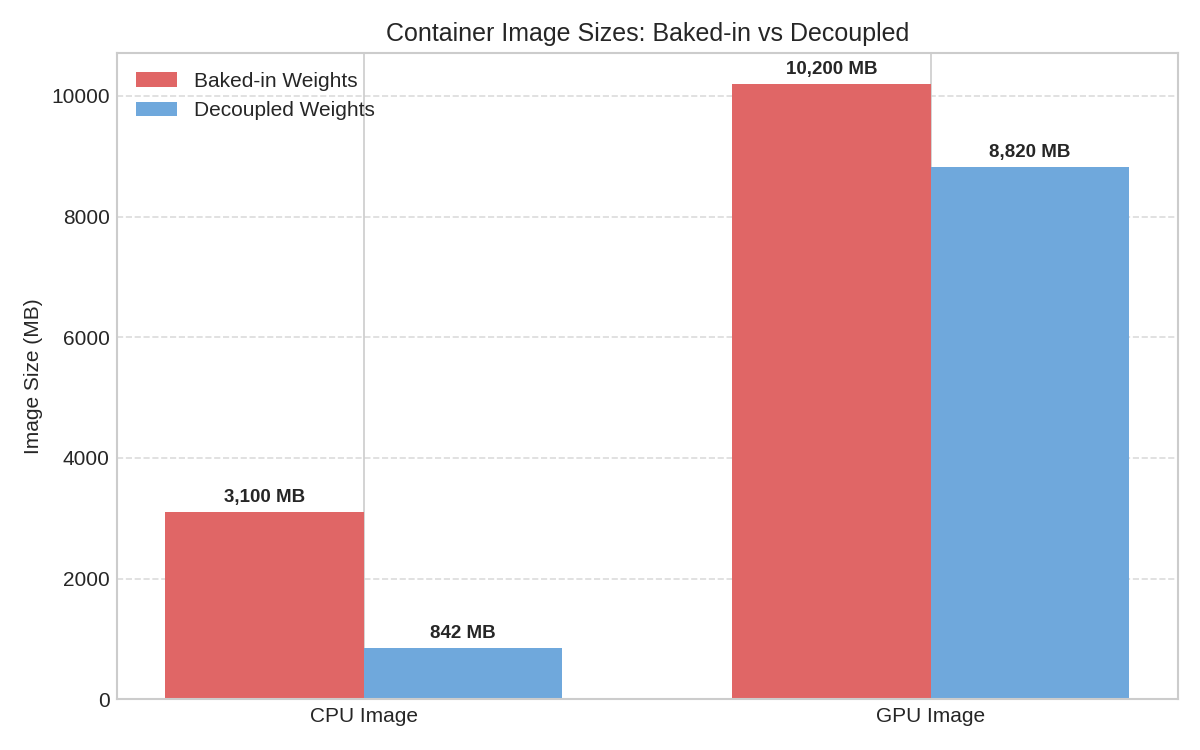
\includegraphics[width=0.85\columnwidth]{outputs/nli_image_footprint.png}
\caption{Container Image Footprint Comparison: Baked-in vs Decoupled Weights.}
\label{fig:footprint}
\end{figure}

\begin{figure}[htbp]
\centering
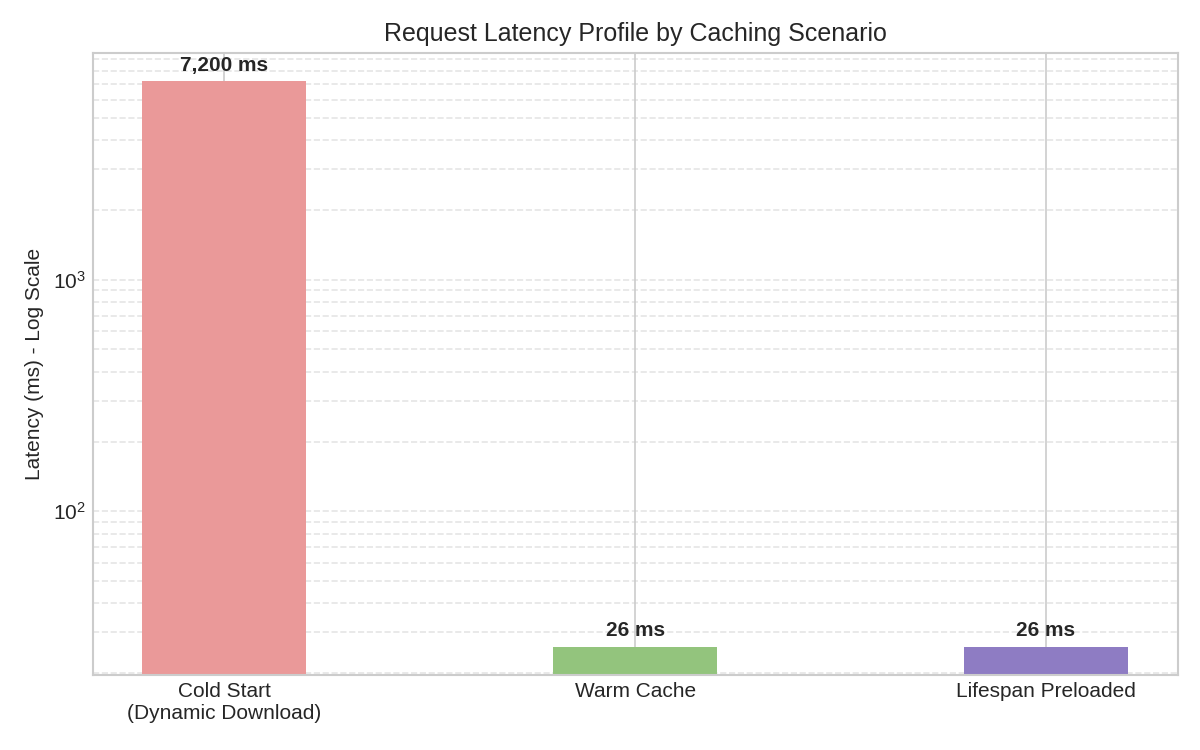
\includegraphics[width=0.85\columnwidth]{outputs/nli_latency_profile.png}
\caption{Scoring Latency Profile across Caching Scenarios.}
\label{fig:latency}
\end{figure}

\end{document}
